\begin{exercise}
      {ID-1ee5508eb879d338143f53a1a03a61730f450df7}
      {Sechseck}
  \ifproblem\problem\par
    Einem Kreis mit Radius $r$ wird ein regelmäßiges Sechseck einbeschrieben und
    ein regelmäßiges Sechseck umbeschrieben.\par
    \begin{minipage}{0.35\textwidth}
      \centering
      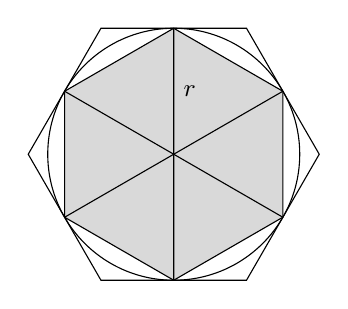
\begin{tikzpicture}[scale=0.8]
        % umbeschriebenes Sechseck
        \begin{scope}[rotate=60]
          \draw (  0:2.31) --
                ( 60:2.31) --
                (120:2.31) --
                (180:2.31) --
                (240:2.31) --
                (300:2.31) -- cycle;
        \end{scope}
        % einbeschriebenes Sechseck
        \begin{scope}[rotate=30]
          \filldraw[fill=black!15!white, draw=black]
                   (  0:2) --
                   ( 60:2) --
                   (120:2) --
                   (180:2) --
                   (240:2) --
                   (300:2) -- cycle;
          \draw (0, 0) -- (  0:2);
          \draw (0, 0) -- ( 60:2);
          \draw (0, 0) -- (120:2);
          \draw (0, 0) -- (180:2);
          \draw (0, 0) -- (240:2);
          \draw (0, 0) -- (300:2);
        \end{scope}
        % Kreis
        \draw (0, 0) circle (2);
        % Beschriftung
        \node[right] at (90:1) {{\small$r$}};
      \end{tikzpicture}
    \end{minipage}\hfill
    \begin{minipage}{0.64\textwidth}
      \begin{enumerate}[a)]
        \item Berechne den Umfang und den Flächeninhalt der beiden Sechsecke in
              Abhängigkeit von $r$.        \item Um wie viel Prozent sind Umfang und Flächeninhalt des einbeschriebenen
              Sechsecks kleiner als die des umbeschriebenen?
      \end{enumerate}
    \end{minipage}
  \fi
  \ifoutline\outline\par
    \begin{enumerate}[a)]
      \item Das einbeschriebe Sechseck besteht aus gleichseitigen
            Dreiecken mit Seitenlänge $r$.
            Das umbeschriebe Sechseck besteht aus gleichseitigen
            Dreiecken mit Höhe $r$.
      \item Beim Bilden der Quotienten lässt sich der Radius kürzen:
            \begin{equation*}
              p\,\%=1-\frac{U_\text{ein}}{U_\text{um}}
              \quad\text{bzw.}\quad
              p\,\%=1-\frac{A_\text{ein}}{A_\text{um}}
            \end{equation*}
    \end{enumerate}
  \fi
  \ifoutcome\outcome\par
    \begin{enumerate}[a)]
      \item Für das einbeschriebe Sechseck gilt:
            \begin{equation*}
              U=6r
              \quad\text{und}\quad
              A=\frac{3}{2}\cdot\sqrt{3}\cdot r^2
            \end{equation*}
            Für das umbeschriebe Sechseck gilt:
            \begin{equation*}
              U=4\cdot\sqrt{3}\cdot r
              \quad\text{und}\quad
              A=2\cdot\sqrt{3}\cdot r^2
            \end{equation*}
      \item Der Umfang des einbeschrieben Sechsecks ist
            ca. \pc{13.4} kürzer als der Umfang des
            umbeschriebenen Sechsecks. Der exakte Wert beträgt
            \begin{equation*}
              1-\frac{\sqrt{3}}{2}
            \end{equation*}
            Der Flächeninhalt des einbeschrieben Sechsecks ist
            \pc{25} kleiner als der Flächeninhalt des
            umbeschriebenen Sechsecks.
    \end{enumerate}
  \fi
\end{exercise}
